\subsection{Estructura de la red telefónica}
Se trata de un sistema con bloqueo, se puede variar con sistemas adicionales como el buzón de voz o similares a un sistema con espera. Cuando era analógica la red telefónica se trataba de un sistema de conmutación de circuitos.\\
Las centrales de conmutaciónse basan en la idea de conmutación multietapa, con esto se evita el tener un cable por destino. La estructura jerarquica de la red telefónica está descrita a continuación:
\begin{itemize}
\item Un par de abonado entre cada cliente y la central local. [CL]
\item Central primaria enlaza 2 o más centrales locales. [CP]
\item Bucle de abonado, del abonado a la central local.
\item Enlace troncal, los internos entre centrales, también llamados enlace final.
\item Central secundaria une dos o más centrales primarias. [CS]
\item Central terciaria y superiores enlazan dos o ás centrales de orden inferior. [CT]
\item Una ruta final está unicamente formada por enlaces finales.
\end{itemize}
\begin{figure}[H]
\centering
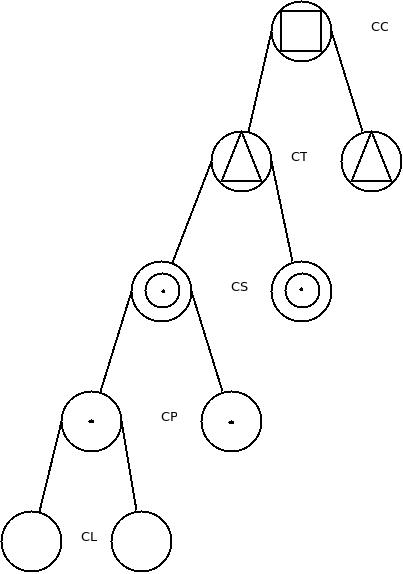
\includegraphics[width=0.9\textwidth]{Imagen/diajerartelefono.jpg}
\caption{Diagrama de la red jerárquica}
\label{diaRedTelefonica}
\end{figure}
A parte de la red jerarquica existe la red complementaria. Esta está formada por enlaces directos. Enlaces que unen centrales que no están unidas jerarquicamente.\\
\subsubsection{Encaminamiento en la estructura de la red telefónica}
\begin{enumerate}
\item Identificamos el arbol de destino. Está formado por todos los nodos jerarquicamente superiores al nodo de destino.
\item En cada nodo vemos si hay una sección directa que nos lleve al arbol de destino. No se pueden tomar 2 secciones directas en la misma ruta. Una sección directa nunca desbordará sobre otra sección directa, siempre desbordará sobre la sección final.
\item una vez en el arbol de destino desciendo jerarquicamente hasta el nodo destino.
\end{enumerate}
Con estos pasos se puede encaminar a traves de cualquier estructura gerárquica.
\begin{example}[Encaminamiento en la red telefónica]
\begin{figure}[H]
\centering
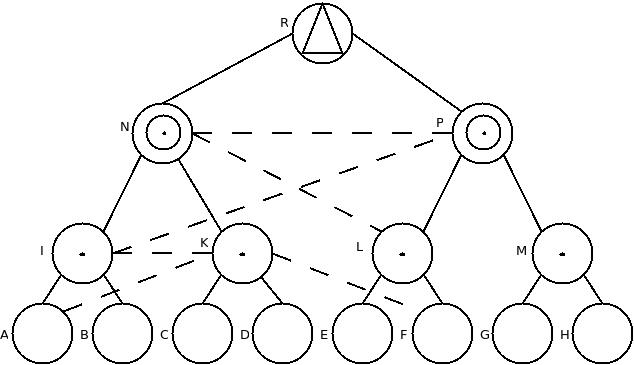
\includegraphics[width=0.9\textwidth]{Imagen/ejemploredtelefonica.jpg}
\label{}
\end{figure}
De la figura podemos sacar las siguientes rutas.\\
\begin{center}
\begin{tabular}{c c c c}
A$\to$C & AKC  		& A$\to$E 	& AIPLE 	\\
 		& AIKC 		&			& AINLE		\\
 		& AINKC		&			& AINRPLE	\\
E$\to$A & ELNIA  	& 		 	& 		 	\\
 		& ELPIA 	&			& 			\\
 		& ELPRNIA	&			& 			\\
\end{tabular}
\end{center}
Como se puede ver no todas las rutas son 100\% simétricas.
\end{example}
\subsubsection{Red inteligente}
Surge con la digitalización y a la vez que la Red Digital de Servicios Integrados (RDSI). Este sistema ofrece servicios de valor añadido.
\begin{figure}[H]
\centering
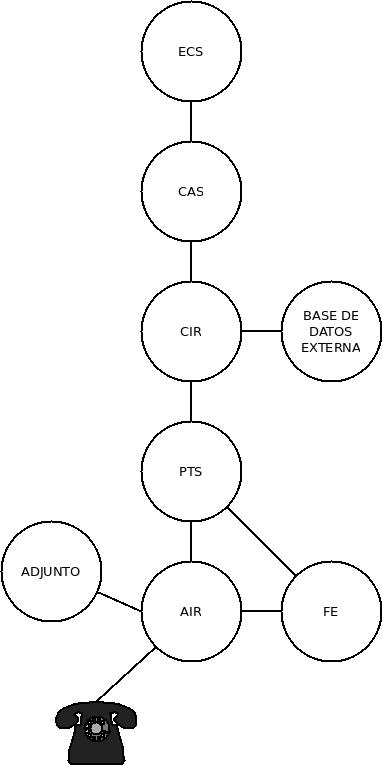
\includegraphics[width=0.5\textwidth]{Imagen/diaredinteligente.jpg}
\caption{Diagrama de la Red Inteligente}
\end{figure}
\begin{itemize}
\item Agencia de Inteligencia de Red [AIR]: Identifica si la llamada está destinada a la Red Inteligente. Solo hay una por Central Local.
\item Punto de Transferencia de Señalización [PTS]: Es un centro de intercambio entre las diferentes partes de la red.
\item Centro de Inteligencia de Red [CIR]: Es la parte más importante de la Red Inteligente ya que es el que reconoce los servicios y da las ordenes.
\item Adjunto: Es como el CIR pero se encuentra en la Central Local. De esta forma descarga las instancias superiores de la red.
\item Módulo de Funciones Especiales [FE]: Cumple varias funciones como la sintesis de voz o la captación de teclas marcadas.
\item Base de datos externa: Se trata de un conjunto de bases de datos que no se encuentran dentro del CIR, como la de tarjetas de crédito.
\item Centro de Administración de Servicios [CAS]: Lugar donde se administra y controla todos los servicios de la red. Este no tiene por que estar conectado a la red constantemente.
\item Entorno de Creación de Servicios [ECS]: Lugar donde se implementan los nuevos servicios. Este no tiene por que estar conectado a la red constantemente.
\end{itemize}